\begin{slikaDesno}{fig/LC.pdf}
{\color{red}*}\PID  У колу са слике познати су 
$L = 100\unit{\upmu H}$ и $C = 1\unit{\upmu F}$.
У почетном тренутку у колу нема 
акумулисане енергије. Посматра
се систем чији је улаз напон побудног генератора $v_{\rm U} = v_{\rm U}(t)$ а излаз напон у колу 
$v_{\rm I} = v_{\rm I}(t)$. 
Познато је $v_{\rm I}(t < 0) = 0$ а побуда
је у облику $v_{\rm U}(t) = V_{\rm m} 
\sin(\upomega t)\,{\rm u}(t)$, где је 
$V_{\rm m} = 10\unit{mV}$. Одредити 
и скицирати напон на 
излазу система када је кружна учестаност 
побудног генератора (а) $\upomega = 10^3 
\unit{\dfrac{rad}{s}}$ и (б) 
$\upomega = 10^5 
\unit{\dfrac{rad}{s}}$. За учестаност из 
тачке (б) скицирати и (в) дијаграм снаге 
коју улаже напонски генератор у колу
$p_{\rm g} =p_{\rm g}(t)$.
\end{slikaDesno}\\

\textsc{\underline{Резултат}}:

(а) Тражени одзив је $v_{\rm I}(t) = 10\unit{mV} \sin(\upomega t)$. 
Резултат је приказан на слици \ref{fig:\ID.a}.\\[2mm]

(б) Тражени одзив је $v_{\rm I}(t) = -0,5\unit{\dfrac{V}{ms}} t \cos(\upomega t)$.
Резултат је приказан на слици \ref{fig:\ID.b}.\\[2mm]

(в) Тражена снага је $p_{\rm g} \approx 250\unit{\dfrac{\upmu W}{ms}} t
\bigl(1 + \cos(2\upomega t) \bigr)$.
Резултат је приказан на слици \ref{fig:\ID.v}. \\

\noindent
\begin{figure}[ht!]
    \hspace*{0pt}%\hfill
    \begin{subfigure}[b]{0.32\textwidth}
        %\centering
        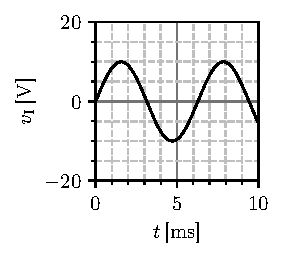
\includegraphics[scale=1]{fig/LC_a.pdf}
        \caption{}
        \label{fig:\ID.a}
    \end{subfigure}
    %\hfill
    \begin{subfigure}[b]{0.32\textwidth}
        %\centering
        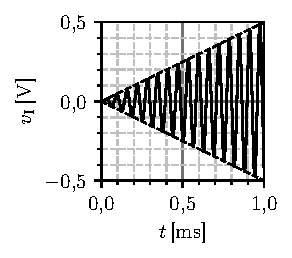
\includegraphics[scale=1]{fig/LC_b.pdf}
        \caption{}
        \label{fig:\ID.b}
    \end{subfigure}
    %\hfill
    \begin{subfigure}[b]{0.32\textwidth}
        %\centering
        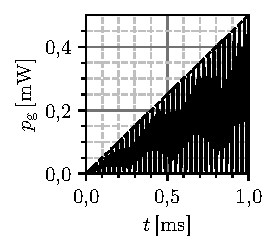
\includegraphics[scale=1]{fig/LC_v.pdf}
        \caption{}
        \label{fig:\ID.v}
    \end{subfigure}
    %\hfill
    %\hspace*{0pt}
    \caption{}
    \label{fig:\ID.2}
\end{figure}



